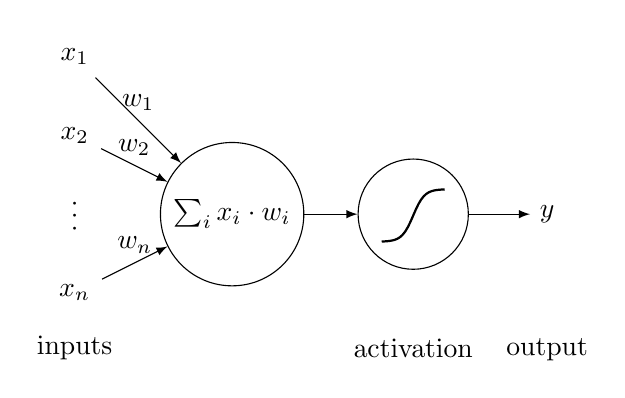
\begin{tikzpicture}[]
\node[circle](x1) at (-2, 2) {$x_1$};
\node[circle](x2) at (-2, 1) {$x_2$};

\node[circle](xn) at (-2, -1) {$x_n$};
\path (x2) -- node[rotate=90]{\ldots} (xn) ;
\node[circle, draw](center) at (0, 0) {$\sum_i x_i \cdot w_i$};
\node[circle, draw, minimum width=1.4cm](activ) at (2.3, 0) {};
\node (output) at (4, 0) {$y$};

\draw[domain=1.9:2.7, thick] plot (\x, {1/(1.5*(1+exp(-14*(\x-2.3)))) - .35});

%\draw[thick] (1.85 , -0.2) --  (2.5, -0.2) -- (2.8, 0.4);

\draw[-latex]  (center) -- (activ);
\draw[-latex] (x1) -- node[above]{$w_1$} (center);
\draw[-latex] (x2) -- node[above]{$w_2$}(center);
\draw[-latex] (xn) -- node[above]{$w_n$}(center);
\draw[-latex] (activ) -- (output);

\node ( ) at (-2,-1.7) {inputs};
\node ( ) at (2.3,-1.7) {activation};
\node ( ) at (4,-1.72) {output};

\end{tikzpicture}
